% Options for packages loaded elsewhere
\PassOptionsToPackage{unicode}{hyperref}
\PassOptionsToPackage{hyphens}{url}
\PassOptionsToPackage{dvipsnames,svgnames*,x11names*}{xcolor}
%
\documentclass[
  8pt,
  ignorenonframetext,
  dvipsnames]{beamer}
\usepackage{pgfpages}
\setbeamertemplate{caption}[numbered]
\setbeamertemplate{caption label separator}{: }
\setbeamercolor{caption name}{fg=normal text.fg}
\beamertemplatenavigationsymbolsempty
% Prevent slide breaks in the middle of a paragraph
\widowpenalties 1 10000
\raggedbottom
\setbeamertemplate{part page}{
  \centering
  \begin{beamercolorbox}[sep=16pt,center]{part title}
    \usebeamerfont{part title}\insertpart\par
  \end{beamercolorbox}
}
\setbeamertemplate{section page}{
  \centering
  \begin{beamercolorbox}[sep=12pt,center]{part title}
    \usebeamerfont{section title}\insertsection\par
  \end{beamercolorbox}
}
\setbeamertemplate{subsection page}{
  \centering
  \begin{beamercolorbox}[sep=8pt,center]{part title}
    \usebeamerfont{subsection title}\insertsubsection\par
  \end{beamercolorbox}
}
\AtBeginPart{
  \frame{\partpage}
}
\AtBeginSection{
  \ifbibliography
  \else
    \frame{\sectionpage}
  \fi
}
\AtBeginSubsection{
  \frame{\subsectionpage}
}
\usepackage{lmodern}
\usepackage{amssymb,amsmath}
\usepackage{ifxetex,ifluatex}
\ifnum 0\ifxetex 1\fi\ifluatex 1\fi=0 % if pdftex
  \usepackage[T1]{fontenc}
  \usepackage[utf8]{inputenc}
  \usepackage{textcomp} % provide euro and other symbols
\else % if luatex or xetex
  \usepackage{unicode-math}
  \defaultfontfeatures{Scale=MatchLowercase}
  \defaultfontfeatures[\rmfamily]{Ligatures=TeX,Scale=1}
\fi
% Use upquote if available, for straight quotes in verbatim environments
\IfFileExists{upquote.sty}{\usepackage{upquote}}{}
\IfFileExists{microtype.sty}{% use microtype if available
  \usepackage[]{microtype}
  \UseMicrotypeSet[protrusion]{basicmath} % disable protrusion for tt fonts
}{}
\makeatletter
\@ifundefined{KOMAClassName}{% if non-KOMA class
  \IfFileExists{parskip.sty}{%
    \usepackage{parskip}
  }{% else
    \setlength{\parindent}{0pt}
    \setlength{\parskip}{6pt plus 2pt minus 1pt}}
}{% if KOMA class
  \KOMAoptions{parskip=half}}
\makeatother
\usepackage{xcolor}
\IfFileExists{xurl.sty}{\usepackage{xurl}}{} % add URL line breaks if available
\IfFileExists{bookmark.sty}{\usepackage{bookmark}}{\usepackage{hyperref}}
\hypersetup{
  pdftitle={Introduction to Multivariate Regression \& Econometrics},
  pdfauthor={Lecture 11},
  colorlinks=true,
  linkcolor=Maroon,
  filecolor=Maroon,
  citecolor=Blue,
  urlcolor=blue,
  pdfcreator={LaTeX via pandoc}}
\urlstyle{same} % disable monospaced font for URLs
\newif\ifbibliography
\usepackage{graphicx,grffile}
\makeatletter
\def\maxwidth{\ifdim\Gin@nat@width>\linewidth\linewidth\else\Gin@nat@width\fi}
\def\maxheight{\ifdim\Gin@nat@height>\textheight\textheight\else\Gin@nat@height\fi}
\makeatother
% Scale images if necessary, so that they will not overflow the page
% margins by default, and it is still possible to overwrite the defaults
% using explicit options in \includegraphics[width, height, ...]{}
\setkeys{Gin}{width=\maxwidth,height=\maxheight,keepaspectratio}
% Set default figure placement to htbp
\makeatletter
\def\fps@figure{htbp}
\makeatother
\setlength{\emergencystretch}{3em} % prevent overfull lines
\providecommand{\tightlist}{%
  \setlength{\itemsep}{0pt}\setlength{\parskip}{0pt}}
\setcounter{secnumdepth}{-\maxdimen} % remove section numbering

%packages
\usepackage{graphicx}
\usepackage{rotating}
\usepackage{hyperref}

\usepackage{tikz} % used for text highlighting, amongst others
\usepackage{comment}

%title slide stuff
%\institute{Department of Education}
%\title{Managing and Manipulating Data Using R}

%
\setbeamertemplate{navigation symbols}{} % get rid of navigation icons:
\setbeamertemplate{footline}[page number]

%\setbeamertemplate{frametitle}{\thesection \hspace{0.2cm} \insertframetitle}
\setbeamertemplate{section in toc}[sections numbered]
%\setbeamertemplate{subsection in toc}[subsections numbered]
\setbeamertemplate{subsection in toc}{%
  \leavevmode\leftskip=3.2em\color{gray}\rlap{\hskip-2em\inserttocsectionnumber.\inserttocsubsectionnumber}\inserttocsubsection\par
}

%define colors
%\definecolor{uva_orange}{RGB}{216,141,42} % UVa orange (Rotunda orange)
\definecolor{mygray}{rgb}{0.95, 0.95, 0.95} % for highlighted text
	% grey is equal parts red, green, blue. higher values >> lighter grey
	%\definecolor{lightgraybo}{rgb}{0.83, 0.83, 0.83}

% new commands

%highlight text with very light grey
\newcommand*{\hlg}[1]{%
	\tikz[baseline=(X.base)] \node[rectangle, fill=mygray] (X) {#1};%
}
%, inner sep=0.3mm
%highlight text with very light grey and use font associated with code
\newcommand*{\hlgc}[1]{\texttt{\hlg{#1}}}

%modifying back ticks to add grey background
\let\OldTexttt\texttt
\renewcommand{\texttt}[1]{\OldTexttt{\hlg{#1}}}


\begin{comment}

% Font
\usepackage[defaultfam,light,tabular,lining]{montserrat}
\usepackage[T1]{fontenc}
\renewcommand*\oldstylenums[1]{{\fontfamily{Montserrat-TOsF}\selectfont #1}}

% Change color of boldface text to darkgray
\renewcommand{\textbf}[1]{{\color{darkgray}\bfseries\fontfamily{Montserrat-TOsF}#1}}

% Bullet points
\setbeamertemplate{itemize item}{\color{BlueViolet}$\circ$}
\setbeamertemplate{itemize subitem}{\color{BrickRed}$\triangleright$}
\setbeamertemplate{itemize subsubitem}{$-$}

% Reduce space before lists
%\addtobeamertemplate{itemize/enumerate body begin}{}{\vspace*{-8pt}}

\let\olditem\item
\renewcommand{\item}{%
  \olditem\vspace{4pt}
}

% decreasing space before and after level-2 bullet block
%\addtobeamertemplate{itemize/enumerate subbody begin}{}{\vspace*{-3pt}}
%\addtobeamertemplate{itemize/enumerate subbody end}{}{\vspace*{-3pt}}

% decreasing space before and after level-3 bullet block
%\addtobeamertemplate{itemize/enumerate subsubbody begin}{}{\vspace*{-2pt}}
%\addtobeamertemplate{itemize/enumerate subsubbody end}{}{\vspace*{-2pt}}

%Section numbering
\setbeamertemplate{section page}{%
    \begingroup
        \begin{beamercolorbox}[sep=10pt,center,rounded=true,shadow=true]{section title}
        \usebeamerfont{section title}\thesection~\insertsection\par
        \end{beamercolorbox}
    \endgroup
}

\setbeamertemplate{subsection page}{%
    \begingroup
        \begin{beamercolorbox}[sep=6pt,center,rounded=true,shadow=true]{subsection title}
        \usebeamerfont{subsection title}\thesection.\thesubsection~\insertsubsection\par
        \end{beamercolorbox}
    \endgroup
}

\end{comment}

\title{Introduction to Multivariate Regression \& Econometrics}
\subtitle{HED 612}
\author{Lecture 11}
\date{}

\begin{document}
\frame{\titlepage}

\begin{frame}
  \tableofcontents[hideallsubsections]
\end{frame}
\begin{frame}[fragile]{Prepare for class}
\protect\hypertarget{prepare-for-class}{}

We'll be using the California Schools Data today; no need to
re-download!

\medskip

\begin{enumerate}
\tightlist
\item
  Download the Lecture 11 PDF and R files for this week

  \begin{itemize}
  \tightlist
  \item
    Place all files in HED612\_SP21
    \textgreater\textgreater\textgreater{} lectures
    \textgreater\textgreater\textgreater{} lecture11
  \end{itemize}
\item
  Open the RProject (should be in your main HED612\_SP21 folder)
\item
  Once the RStudio window opens, open the Lecture 11 R script by
  clicking on:

  \begin{itemize}
  \tightlist
  \item
    file \textgreater\textgreater\textgreater{} open file\ldots{}
    \textgreater\textgreater\textgreater{} {[}navigate to lecture 11
    folder{]} \textgreater\textgreater\textgreater{} lecture11.R
  \end{itemize}
\item
  \textbf{Install the ``RCurl'' package in Lecture11.R}

  \begin{itemize}
  \tightlist
  \item
    If R prompts you to install \texttt{RCurl} and ``its dependencies'',
    go ahead and click install
  \item
    If R doesn't prompt you, install via line 9
    \texttt{install.packages("RCurl")}
  \end{itemize}
\end{enumerate}

\end{frame}

\begin{frame}{Where are we going\ldots.}
\protect\hypertarget{where-are-we-going.}{}

\begin{itemize}
\tightlist
\item
  Last Two Weeks:

  \begin{itemize}
  \tightlist
  \item
    Moved from bivariate to multivariate regression!
  \item
    How to avoid violating OLS Assumption 1

    \begin{itemize}
    \tightlist
    \item
      Include variables that would result in omitted variable bias
    \end{itemize}
  \end{itemize}
\end{itemize}

\medskip

\begin{itemize}
\tightlist
\item
  This Week:

  \begin{itemize}
  \tightlist
  \item
    Other OLS assumptions
  \item
    Some more multivariate regression practice
  \item
    Reading Empirical Work:

    \begin{itemize}
    \tightlist
    \item
      Powers, J. M. (2004). High-Stakes Accountability and Equity: Using
      Evidence From California's Public Schools Accountability Act to
      Address the Issues in Williams v. State of California. American
      Educational Research Journal, 41(4), 763--795.
    \end{itemize}
  \end{itemize}
\end{itemize}

\end{frame}

\begin{frame}{No Class Next Week: Final Project Meetings}
\protect\hypertarget{no-class-next-week-final-project-meetings}{}

\begin{itemize}
\tightlist
\item
  Next Week 4/7: No Class!

  \begin{itemize}
  \tightlist
  \item
    We're going to use the extra time to get started on final projects!
  \item
    Instead of meeting for class: schedule at least a 30 min meeting
    with me!

    \begin{itemize}
    \tightlist
    \item
      Formulating RQ
    \item
      Operationalizing and cleaning variables
    \end{itemize}
  \item
    Link to sign up: \url{https://calendly.com/ksalazar_az/30min}
  \item
    Submit PS11 after you have met with me!
  \end{itemize}
\end{itemize}

\medskip

\begin{itemize}
\item
  Following Week 4/14:

  \begin{itemize}
  \tightlist
  \item
    Introduction to data transformations

    \begin{itemize}
    \tightlist
    \item
      Logs and Polynomials
    \end{itemize}
  \item
    Introduction to non-linear relationships between X and Y
  \item
    Mini lesson on what each section of final project (Intro, Lit
    Review, Conceptual Framework, etc.) should accomplish!
  \item
    Tutorial on automatic publication ready regression tables in R
  \end{itemize}
\end{itemize}

\end{frame}

\hypertarget{ols-assumptions}{%
\section{OLS Assumptions}\label{ols-assumptions}}

\begin{frame}{OLS Assumptions}
\protect\hypertarget{ols-assumptions-1}{}

\begin{enumerate}
\tightlist
\item
  The conditional assumption of \(u_i\) given \(X_i\) has a mean of zero
\item
  (\(X_i\), \(Y_i\)), \(i=1, ...n\) are independently and identically
  distributed (i.i.d)
\item
  Large outliers are unlikely
\item
  Homoskedasticity
\end{enumerate}

\medskip

\begin{itemize}
\tightlist
\item
  If these assumptions hold:

  \begin{itemize}
  \tightlist
  \item
    Then our OLS estimators, \(\hat{\beta_0}\),
    \(\hat{\beta_1}\)\ldots{}\(\hat{\beta_k}\), have normal
    distributions in large samples
  \item
    And because they have normal distributions, we can use
    \(\hat{\beta_0}\), \(\hat{\beta_1}\)\ldots{}\(\hat{\beta_k}\), to
    test hypothesess about the population parameters \(\beta_0\),
    \(\beta_1\)\ldots{}\(\beta_k\)
  \end{itemize}
\item
  If these assumptions are violated:

  \begin{itemize}
  \tightlist
  \item
    We produced inefficeint and biased estimates, \(\hat{\beta_0}\) and
    \(\hat{\beta_1}\), of the population parameters \(\beta_0\) and
    \(\beta_1\)
  \end{itemize}
\end{itemize}

\end{frame}

\begin{frame}{Second OLS Assumption}
\protect\hypertarget{second-ols-assumption}{}

\begin{enumerate}
\setcounter{enumi}{1}
\tightlist
\item
  \textbf{(\(X_i\), \(Y_i\)), \(i=1, ...n\) are independently and
  identically distributed (i.i.d)}
\end{enumerate}

\begin{itemize}
\tightlist
\item
  What does this mean?

  \begin{itemize}
  \tightlist
  \item
    This is about sampling!
  \end{itemize}
\end{itemize}

\medskip

\emph{(\(X_i\), \(Y_i\)), \(i=1, ...n\) are independently distributed}

\begin{itemize}
\tightlist
\item
  In words: Knowing that observation i takes on particular values for X
  and Y tells you nothing about the probability of the next observation
  taking on particular values for X and Y
\item
  When is assumption of independently distributed violated?

  \begin{itemize}
  \tightlist
  \item
    Longitudinal data: knowing a data point in one time period tells you
    something about a data point in another time period.

    \begin{itemize}
    \tightlist
    \item
      Ex: Amount of \$ student received via a Federal Pell Grant
      freshman year at UA probably tells you something about how much \$
      student received via a Federal Pell Grant sophmore year at UA.
      Why? because Pell status is not likely to dramatically change from
      one year to another!
    \end{itemize}
  \item
    Hierarchical data:

    \begin{itemize}
    \tightlist
    \item
      Ex: Students are nested within classrooms. Knowing the reading
      test score of one student in a classroom is probably correlated
      with reading test score for another student in the same classroom.
    \end{itemize}
  \end{itemize}
\item
  Our course focuses on cross-sectional data (i.e., at one point in
  time); using OLS linear regression for cross-sectional data does not
  violate OLS Assumption \#2
\item
  Time Series and Hierarchical regression modeling is just one
  additional step from regression modeling you have learned in this
  course!

  \begin{itemize}
  \tightlist
  \item
    May create a survey course next academic year that applies what we
    have learned in this course to learning some of these more
    ``complex'' linear models!
  \end{itemize}
\end{itemize}

\end{frame}

\begin{frame}{Second OLS Assumption cont.}
\protect\hypertarget{second-ols-assumption-cont.}{}

\emph{(\(X_i\), \(Y_i\)), \(i=1, ...n\) are identically distributed}

\begin{itemize}
\tightlist
\item
  Prior to choosing sample of observations for the population, the
  probability distribution (i.e., the likelihood that \(Y_i\) takes on
  certain values) is the same for all observations
\item
  This is always true if you take a random sample!

  \begin{itemize}
  \tightlist
  \item
    One randomly selected observation has the same probability of taking
    on a certain value of \(Y_i\) as another randomly selected
    observation
  \end{itemize}
\item
  When is the assumption of identically distributed violated?

  \begin{itemize}
  \tightlist
  \item
    Sampling bias:

    \begin{itemize}
    \tightlist
    \item
      Ex: You want to investigate probability of being tardy to college
      lectures and take a sample of students living on campus. Sampling
      bias: you did not include commuter students. If you were to
      randomly select a student living on campus, they are not likely to
      have the same probability of being tardy to lecture than a
      randomly selected commuter student.
    \end{itemize}
  \end{itemize}
\end{itemize}

\end{frame}

\begin{frame}{Third OLS Assumption}
\protect\hypertarget{third-ols-assumption}{}

\begin{enumerate}
\setcounter{enumi}{2}
\tightlist
\item
  Large outliers are unlikely
\end{enumerate}

\begin{itemize}
\tightlist
\item
  Outliers: observations with values of \(X_i\) and \(Y_i\) that are
  outside the ``usual'' range of the data
\item
  Outliers will affect your regression coefficients!
\item
  Why? Because outliers will shift our OLS regression line!
\end{itemize}

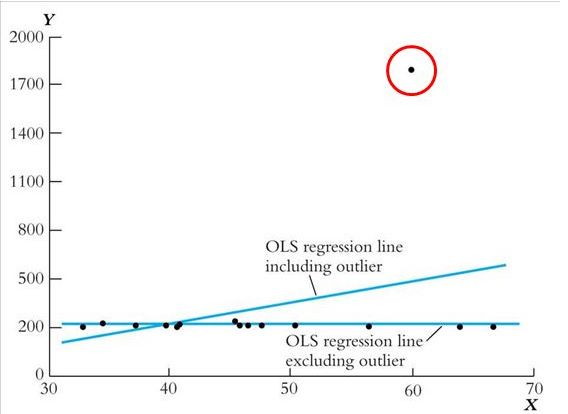
\includegraphics[width=0.85\textwidth,height=\textheight]{outliers.jpg}

\end{frame}

\begin{frame}{Third OLS Assumption cont.}
\protect\hypertarget{third-ols-assumption-cont.}{}

\begin{itemize}
\tightlist
\item
  Stock and Watson have a very technical, mathematical definition of
  when this likely; but in practice this is about really
  investigating/knowing your data
\item
  In practice, if you do find outliers:

  \begin{itemize}
  \tightlist
  \item
    Be sure the data is entered correctly and cleaned

    \begin{itemize}
    \tightlist
    \item
      Ex: Survey data codes missing data as very unusual values (-99,
      -99, 99, 98)
    \end{itemize}
  \item
    Sometimes outliers can belong in the data!
  \item
    If they belong; use natural log of the variable {[}we'll learn more
    about this next week via data transformations!{]}

    \begin{itemize}
    \tightlist
    \item
      Ex: All money variables are usually converted to their natural log
      in econometrics or education research (e.g., state appropriations,
      tuition revenue, household income)
    \end{itemize}
  \end{itemize}
\end{itemize}

\end{frame}

\begin{frame}{Fourth OLS Assumption {[}Not in Stock \& Watson{]}}
\protect\hypertarget{fourth-ols-assumption-not-in-stock-watson}{}

\begin{enumerate}
\setcounter{enumi}{3}
\tightlist
\item
  Homoskedasticity
\end{enumerate}

\begin{itemize}
\tightlist
\item
  There is ``generally'' a fourth OLS assumption, but Stock and Watson
  do not list it in our textbook

  \begin{itemize}
  \tightlist
  \item
    I'll tell you why after we understand what it generally
    assumes\ldots{}
  \end{itemize}
\item
  OLS Assumption \#4: The distribution of the residuals has constant
  variance (homoscedasticity)
\item
  Homoskedasticity

  \begin{itemize}
  \tightlist
  \item
    The distribution (the variance!) of the residuals,
    \(u_i = Y_i - \hat{Y_i}\), is constant for all observations. That
    is, it does not change for different values of X
  \item
    Homo-skedasticity = ``equal'' or ``same'' variances
  \end{itemize}
\item
  Heteroskedasticity

  \begin{itemize}
  \tightlist
  \item
    The distribution (the variance!) of the residuals,
    \(u_i = Y_i - \hat{Y_i}\), is not constant for all observations.
    That is, it does change/differs for different values of X
  \item
    Hetero-skedasticity = ``unequal'' or ``different'' variances
  \end{itemize}
\end{itemize}

\end{frame}

\begin{frame}{Fourth OLS Assumption cont.}
\protect\hypertarget{fourth-ols-assumption-cont.}{}

\begin{itemize}
\tightlist
\item
  Homoskedasticity and Heteroskedasticity shown graphically
\end{itemize}

\end{frame}

\begin{frame}{Fourth OLS Assumption cont.}
\protect\hypertarget{fourth-ols-assumption-cont.-1}{}

\begin{itemize}
\tightlist
\item
  Practical example: What is the effect of student-teacher ratio on test
  scores? {[}Stock and Watson Example{]}
\end{itemize}

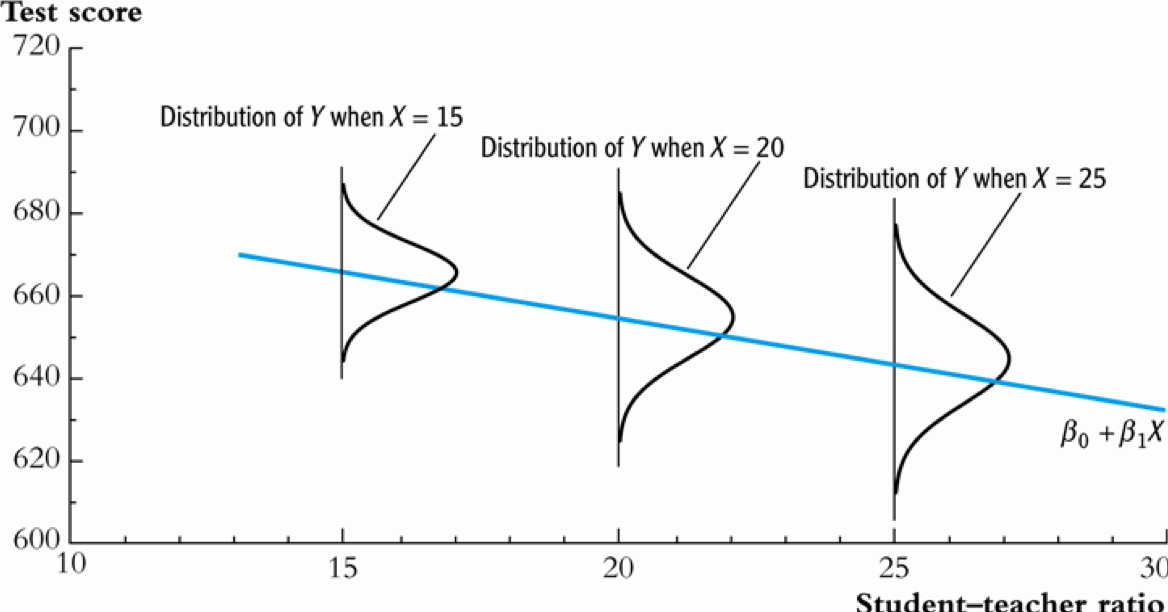
\includegraphics{heteroskedasticity_str.png}

\end{frame}

\begin{frame}{Fourth OLS Assumption cont.}
\protect\hypertarget{fourth-ols-assumption-cont.-2}{}

\begin{itemize}
\tightlist
\item
  Why is homoskedasticity/heteroskedasticity important?

  \begin{itemize}
  \tightlist
  \item
    Because our formula for calculating SE(\(\hat{\beta_1}\)) changes
    based on homoskedastic or heteroskedastic residuals!
  \item
    Our standard error measures how far our \(\hat{\beta_1}\) is likely
    to be from \(\beta_1\). In other words, it is used to calculate our
    t-value in hypothesis testing to determine statistical significance!
  \end{itemize}
\item
  In other statistics classes (non-econometrics), homoskedasticity is
  the fourth core assumption

  \begin{itemize}
  \tightlist
  \item
    Stock and Watson only discuss the first three assumptions as core
    ``OLS Assumptions''
  \end{itemize}
\item
  Why? Stock and Watson say:

  \begin{itemize}
  \tightlist
  \item
    It is NEARLY IMPOSSIBLE to assume homoskedasticity; we almost always
    violate this assumption!
  \item
    But the solution to overcome this assumption is easy!

    \begin{itemize}
    \tightlist
    \item
      We can just calculate heteroskedastic standard errors
    \item
      In other words, standard errors that are \textbf{robust} to
      violations of homoskedasticity
    \end{itemize}
  \end{itemize}
\item
  Stock and Watson say:

  \begin{itemize}
  \tightlist
  \item
    Rather than make homoskedasticity a core OLS Assumption and nearly
    always violate it;
  \item
    ALWAYS CALCULATE ROBUST STANDARD ERRORS AND DO NOT MAKE
    HOMOSKEDASTICITY A CORE OLS ASSUMPTION
  \item
    Show in R
  \end{itemize}
\end{itemize}

\end{frame}

\hypertarget{multivariate-regression-homework-review}{%
\section{Multivariate regression (Homework
Review)}\label{multivariate-regression-homework-review}}

\begin{frame}{Multivariate Regression Example}
\protect\hypertarget{multivariate-regression-example}{}

RQ: What is the effect of student-teacher ratio on reading test scores?

\medskip

Population Regression Model:

\begin{itemize}
\tightlist
\item
  \(Y_i = \beta_0 + \beta_1X_{1i} + \mu_i\)

  \begin{itemize}
  \tightlist
  \item
    Where:
  \item
    \(Y\) = average district reading scores
  \item
    \(X_{1}\) = average district student teacher ratio
  \end{itemize}
\item
  Let's add a categorical ELL variable

  \begin{itemize}
  \tightlist
  \item
    OVB: (1) ELL students are likley to score at lower reading levels
    than native english speakers; (2) \textbf{and} Greater proportion of
    ELL students require smaller class sizes
  \item
    Categories: Low ELL District (0-20\%); Moderate ELL District
    (21-50\%); High ELL District (51\%+)
  \end{itemize}
\item
  Let's also add continuous expenditures per student

  \begin{itemize}
  \tightlist
  \item
    OVB: (1) Districts with greater expenditures per student likely to
    have higher test scores (2) \textbf{and} Greater expenditures per
    student greater spending on teacher salaries and smaller class sizes
  \end{itemize}
\end{itemize}

\end{frame}

\begin{frame}{Multivariate Regression Example}
\protect\hypertarget{multivariate-regression-example-1}{}

RQ: What is the effect of student-teacher ratio on reading test scores?

\medskip

Population Regression Model:

\begin{itemize}
\tightlist
\item
  \(Y_i = \beta_0 + \beta_1X_{1i} + + \beta_2X_{2i} + + \beta_3X_{3i} + \beta_4X_{4i} + \mu_i\)

  \begin{itemize}
  \tightlist
  \item
    \(Y\) = average district reading scores
  \item
    \(X_{1}\) = average district student teacher ratio
  \item
    \(X_{2}\) = 0/1 Moderate ELL District (21-50\%); reference group is
    Low ELL District (0-20\%)
  \item
    \(X_{3}\) = 0/1 High ELL District (51\%+); reference group is Low
    ELL District (0-20\%)
  \item
    \(X_{4}\) = average district expenditures per student (\$000s)
  \end{itemize}
\item
  Create variables and run regression in R!
\end{itemize}

\end{frame}

\begin{frame}{Multivariate Regression Example}
\protect\hypertarget{multivariate-regression-example-2}{}

RQ: What is the effect of student-teacher ratio on reading test scores?

\begin{itemize}
\tightlist
\item
  OLS Line without estimates

  \begin{itemize}
  \tightlist
  \item
    \(\hat{Y_i} = \hat{\beta_0} + \hat{\beta_1}X_{1i} + + \hat{\beta_2}X_{2i} + + \hat{\beta_3}X_{3i} + \hat{\beta_4}X_{4i}\)
  \item
    \(\hat{Y_i} = \hat{\beta_0} + \hat{\beta_1}STR + \hat{\beta_2}ModerateELL + \hat{\beta_3}HighELL + \hat{\beta_4}Expend000\)
  \end{itemize}
\item
  OLS Line with estimates

  \begin{itemize}
  \tightlist
  \item
    \(\hat{Y_i} = 649.03 - (0.68*STR) - (22.31*ModerateELL) - (37.57*HighELL) + (4.94*Expend000)\)
  \end{itemize}
\item
  Interpreting Student-Teacher-Ratio as our IV of interest:

  \begin{itemize}
  \tightlist
  \item
    On average, one additional student per teacher (``one unit
    increase'') in district average student-teacher-ratio is associated
    with 0.68 point decrease in average district reading scores, holding
    the values of covariates constant. However, our coefficient is not
    significant at the 0.05 level.
  \end{itemize}
\item
  Interpreting ELL as our IV of interest:

  \begin{itemize}
  \tightlist
  \item
    On average, being a ``Moderate ELL district'' as opposed to a ``Low
    ELL district'' is associated with 22.31 point decrease in reading
    scores (p\textless0.001), holding the values of covariates constant.
  \item
    On average, being a ``High ELL district'' as opposed to a ``Low ELL
    district'' is associated with 37.57 point decrease in reading scores
    (p\textless0.001), holding the values of covariates constant.
  \end{itemize}
\item
  Interpreting Expenditures Per Student as our IV of interest:

  \begin{itemize}
  \tightlist
  \item
    On average, a \$1000 increase (``one unit increase'') in
    expenditures per student is associated with 4.95 point increase in
    average district reading scores (p\textless0.01), holding the values
    of covariates constant.
  \end{itemize}
\end{itemize}

\end{frame}

\hypertarget{minute-break}{%
\section{10 Minute Break!}\label{minute-break}}

\hypertarget{learning-to-read-quantitative-empirical-work}{%
\section{Learning to Read Quantitative Empirical
Work}\label{learning-to-read-quantitative-empirical-work}}

\begin{frame}{Powers (2004): Overall RQ, Analytical and Writting
Approach!}
\protect\hypertarget{powers-2004-overall-rq-analytical-and-writting-approach}{}

\begin{itemize}
\tightlist
\item
  \textbf{Williams v. State of California}

  \begin{itemize}
  \tightlist
  \item
    Class action lawsuit against the State of California in 2000; public
    school students represented by a coalition of law firms, civil
    rights organizations
  \item
    Argued that if schools and students are judged on the basis of their
    test scores (high stakes accountability policies), then students and
    schools should be provided with equal access to school-related
    resources needed for academic success
  \item
    Specifically addressed need for qualified teachers,
    sufficient/up-to-date textbooks, and adequate/safe facilities
  \end{itemize}
\item
  \textbf{Old legal approach to school financing}: focused on levels and
  formulas of spending

  \begin{itemize}
  \tightlist
  \item
    Didn't work because the state has minimal oversight of local
    educational control/``property taxes''; caps were eliminated via
    voter overrides; and the small proportion of state funding was given
    ``equally''
  \end{itemize}
\item
  \textbf{New legal approach to school financing}: \emph{Williams v.
  State of California} reframed the issue of school financing around the
  \emph{conditions} of education rather than funding formulas!

  \begin{itemize}
  \tightlist
  \item
    Worked because the state is responsible for ensuring resources are
    used to produce desirable outcomes
  \end{itemize}
\item
  State of California argued that there was little empirical support
  that increased spending on resources identified in the case would
  increase student achievement

  \begin{itemize}
  \tightlist
  \item
    \textbf{RQ}: What is the relationship(s) between school and district
    characteristics on school's academic performance?
  \end{itemize}
\end{itemize}

\end{frame}

\begin{frame}{Powers (2004): Overall RQ, Analytical and Writting
Approach!}
\protect\hypertarget{powers-2004-overall-rq-analytical-and-writting-approach-1}{}

\begin{itemize}
\tightlist
\item
  \textbf{Empirical Strategy}

  \begin{itemize}
  \tightlist
  \item
    Powers is not trying to establish a causal effect of school/resource
    characteristics on API score explicitly (impossible given the
    observational data)
  \item
    But she is trying to isolate the Williams Case variables
    ``relationship'' on schools' academic performance by controlling for
    other factors that may be driving variation in schools' academic
    performance!

    \begin{itemize}
    \tightlist
    \item
      See on See pg.766 for rationale in including control variables
    \item
      ``To ensure the findings related to Williams variables are robust,
      that is, they are not systematically related to student, school,
      and district characteristics''
    \end{itemize}
  \item
    But still analyzing ``descriptive relationships'', not ``causal
    relationships''
  \end{itemize}
\item
  \textbf{Literature Review Strategy}

  \begin{itemize}
  \tightlist
  \item
    HOW you format your literature review depends on your RQ and what is
    substantively important
  \end{itemize}

  \begin{enumerate}
  [(1)]
  \tightlist
  \item
    Focus on reviewing scholarship about your X (most econometrics
    studies do this)

    \begin{itemize}
    \tightlist
    \item
      Ex: What is the effect of receiving a Pell Grant on achievement?;
      review scholarship on the effect of Pell grants on all student
      outcomes (GPA, graduation, labor market, etc.)
    \end{itemize}
  \item
    Focus on reviewing scholarship about your Y (many
    prediction/descriptive studies do this)

    \begin{itemize}
    \tightlist
    \item
      EX: What is the (predicted) probability of a student persisting
      into their 2nd year of college?; review scholarship on what we
      know about persistence (more likely to persist if you're involved
      on campus, live on campus, etc.)
    \end{itemize}
  \item
    Focus on reviewing scholarship that specifically speaks to the
    \emph{relationship} between X and Y

    \begin{itemize}
    \tightlist
    \item
      Ex: POWERS (2004, p.772): What do we know about the relationship
      between school resources and academic achievement
    \end{itemize}
  \end{enumerate}
\end{itemize}

\end{frame}

\begin{frame}{Powers (2004)}
\protect\hypertarget{powers-2004}{}

\begin{itemize}
\tightlist
\item
  \textbf{Data}: California DOE Data, school-level; Census Data; Federal
  School Data

  \begin{itemize}
  \tightlist
  \item
    Dependent variable(s): ?
  \item
    Independent variable(s) of interest: ?

    \begin{itemize}
    \tightlist
    \item
      Hint there are three groupings and they are related to the
      Williams Case
    \end{itemize}
  \item
    Control Variables: ?

    \begin{itemize}
    \tightlist
    \item
      Hint there are two groupings!
    \item
      Some control variables left out due to ``collinearity''
    \item
      \textbf{Collinearity}: When two or more of your independent
      variables are highly correlated; so correlated that adding just
      one of them explains both of their ``effect'' on the dependent
      variable. In other words including BOTH independent variables that
      are highly correlated is redundant and takes up statistical power
    \item
      R will automatically drop variables if there is collinearity!
    \end{itemize}
  \end{itemize}
\item
  \textbf{Model}: OLS Linear Regression

  \begin{itemize}
  \tightlist
  \item
    Powers doesn't write out the equation for the study!
  \item
    Let's write it ourselves! {[}at least for the three groups of
    variables for Williams Case{]}
  \end{itemize}
\end{itemize}

\end{frame}

\begin{frame}{Powers (2004)}
\protect\hypertarget{powers-2004-1}{}

\begin{itemize}
\tightlist
\item
  Table 2: Nested Regression Models Using 1999 API Index as DV, pg. 781

  \begin{itemize}
  \tightlist
  \item
    The most ``standard way'' to format regression results
  \item
    You show the ``progression'' towards your final regression model via
    multiple models

    \begin{itemize}
    \tightlist
    \item
      Intercept-only model (no independent variables) {[}Powers didnt
      show this{]}
    \item
      Model 1 can have your independent variable of interest (standard
      for program eval) or some variables (Powers did student
      characteristics)
    \item
      Models 2+\ldots{} shows the addition of control variables
    \end{itemize}
  \item
    Shows beta coefficients, standard errors, and significant levels!
  \end{itemize}
\item
  Does show model fit statistics!

  \begin{itemize}
  \tightlist
  \item
    Powers is not writing from a program evaluation standpoint
  \item
    Rather she's trying to show how variables from Williams Case explain
    (predict!) API scores
  \item
    In this case, measures of model fit are important
  \item
    \(R^2\) increases from Model 1 to Model 2

    \begin{itemize}
    \tightlist
    \item
      Change in \(R^2\) doesn't mean that Williams case IVs add
      ``little'' explanation; see pg 782!
    \end{itemize}
  \item
    In text, she mentions overall F-test is significant from Model 1 to
    Model 2
  \item
    F-test is related to \(R^2\)

    \begin{itemize}
    \tightlist
    \item
      \(H_0\): model with no independent variables (or limited IVs) fits
      the data just as well as model with full variables
    \item
      \(H_a\): model with more variables fits the data better than model
      with no IVs
    \end{itemize}
  \end{itemize}
\end{itemize}

\end{frame}

\begin{frame}{Powers (2004)}
\protect\hypertarget{powers-2004-2}{}

\begin{itemize}
\tightlist
\item
  Interpretation for Table 2 for Williams Case Variables
\item
  In text, she hardly interprets beta coefficients beyond ``significance
  and direction''

  \begin{itemize}
  \tightlist
  \item
    Only sometimes mentions the magnitude of the coefficient
  \item
    This approach is common in ``descriptive research''
  \end{itemize}
\item
  \textbf{Teacher training} (reference group is fully credentialed
  teachers)

  \begin{itemize}
  \tightlist
  \item
    \textbf{Emergency Credentialed \(\hat{\beta}\) Coefficient: -1.12***
    SE= 0.09}

    \begin{itemize}
    \tightlist
    \item
      Interpretation: ``On average, one-percentage-point increase in a
      school teaching staff's proportion of emergency credentialed
      teachers (as opposed to fully credentialed teachers) is associated
      with a 1.12 point decrease in API score, holding all covariates
      constant''
    \end{itemize}
  \end{itemize}
\item
  \textbf{Teacher Experience}

  \begin{itemize}
  \tightlist
  \item
    \textbf{Years teaching \(\hat{\beta}\) Coefficient: .80** SE= 0.26}

    \begin{itemize}
    \tightlist
    \item
      Interpretation: ``A one year increase in a school teaching staff's
      average years of experience, on average, is associated with a 0.80
      point increase in API score, holding all covariates constant''\\
    \end{itemize}
  \end{itemize}
\item
  \textbf{Teacher Education} (reference group is less than M.A)

  \begin{itemize}
  \tightlist
  \item
    \textbf{Greater than MA \(\hat{\beta}\) Coefficient: .42*** SE=
    0.06}

    \begin{itemize}
    \tightlist
    \item
      Interpretation: ``On average, a one-percentage-point increase in a
      school teaching staff's proportion of teachers with greater than
      MA degree (as opposed to lower than MA teachers) is associated
      with a 0.42 point increase in API score, holding all covariates
      constant''
    \end{itemize}
  \end{itemize}
\item
  \textbf{School Calendar} (reference group is traditional year)

  \begin{itemize}
  \tightlist
  \item
    \textbf{Concept 6 \(\hat{\beta}\) Coefficient: -34.46*** SE= 4.52}

    \begin{itemize}
    \tightlist
    \item
      Interpretation: ``On average, being a school with a Concept 6
      Calendar as opposed to a Traditional Calendar is associated with a
      34.46 point decrease in API score, holding all covariates
      constant''
    \end{itemize}
  \end{itemize}
\item
  \textbf{Textbooks}

  \begin{itemize}
  \tightlist
  \item
    \textbf{Per-pupil textbook expenditures \(\hat{\beta}\) Coefficient:
    .11*** SE=0.003}

    \begin{itemize}
    \tightlist
    \item
      Interpretation: ``A \$1 increase in per-pupil expenditures for
      textbooks is associated with a 0.1 point increase in API score,
      holding all covariates constant''\\
    \item
      Interpretation: ``A \$10 increase in per-pupil expenditures for
      textbooks, on average, is associated with a 1 point increase in
      API score, holding all covariates constant''\\
    \item
      Interpretation: ``A \$100 increase in per-pupil expenditures for
      textbooks, on average, is associated with a 10 point increase in
      API score, holding all covariates constant''
    \end{itemize}
  \end{itemize}
\end{itemize}

\end{frame}

\begin{frame}{Powers (2004)}
\protect\hypertarget{powers-2004-3}{}

Why do I like this piece of scholarship?

\begin{itemize}
\tightlist
\item
  The methods are simple!

  \begin{itemize}
  \tightlist
  \item
    Impactful research does not need to have complex methods!
  \item
    Study does not use any analyses/methods beyond what we have learned
    so far in an introductory regression class; yet it is published in
    the AERA flagship journal
  \end{itemize}
\item
  Example of how to deal with ``metrics'' that I fundamentally disagree
  with but are part of our educational reality

  \begin{itemize}
  \tightlist
  \item
    Metrics like SAT/ACT scores, standardized K-12 test, are ``firmly
    entrenched part of the political landscape'' that schools and
    students must navigate
  \item
    In many cases, they are institutionalized within federal, state, and
    university/school policies
  \item
    ``Aim is to make a strong argument for equity by marshaling the very
    data that dominate the political discourse'' (p.~765)
  \end{itemize}
\item
  Direct response to policies
\item
  Cool understanding of legal logic when it comes to education finance!
\end{itemize}

\end{frame}

\end{document}
